% @Author: AnthonyKenny98
% @Date:   2020-04-08 18:12:53
% @Last Modified by:   AnthonyKenny98
% @Last Modified time: 2020-04-09 08:37:24
\begin{figure}[H]
\begin{centering}
\begin{tabular}{c}

\begin{subfigure}{\linewidth}
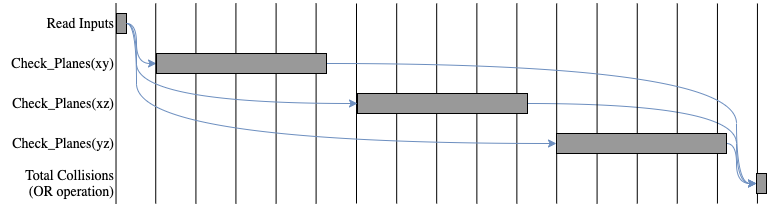
\includegraphics[width=\linewidth]{chapters/chapter3/img/timing1.png}
\caption{HoneyBee-A Timing Diagram. \texttt{Check\_Planes} executed sequentially.}
\label{fig:hbb_timing_a}
\end{subfigure} \\

\begin{subfigure}{\linewidth}
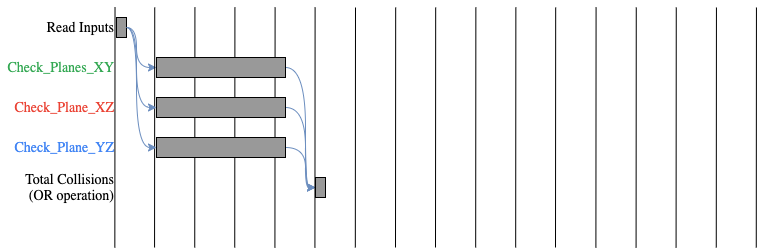
\includegraphics[width=\linewidth]{chapters/chapter3/img/timing2.png}
\caption{HoneyBee-B Timing Diagram. \texttt{Check\_Planes} executed in parallel. Different colors are to represent slightly different implementations of the same function.}
\label{fig:hbb_timing_b}
\end{subfigure} \\

\end{tabular}
\mycaption{Timing Diagrams Showing Parallelization in HoneyBee-B}{. Note, these are simlified timing diagrams for easy explanation of the concept of hardware parallelization.}
\label{fig:hbb_timing}
\end{centering}
\end{figure}